\title{Assessing the Reliability \\of\\ Applications with Supervision Tree}
\author{ Jiansen HE }

% \date{\today}
\date{}
\documentclass[12pt, authoryear]{article}

\usepackage{comment}
\usepackage{natbib} 
%% \usepackage[style=alphabetic]{biblatex}
%% \usepackage[authoryear]{natbib}
%% \PassOptionsToPackage{authoryear}{natbib}
%% \usepackage{caption}
\usepackage{graphicx}
\usepackage{subfigure}
\usepackage{subcaption}
\usepackage{url}

\usepackage{paralist}
\usepackage[pdfpagelabels]{hyperref}
\usepackage[all]{hypcap}
\usepackage{verbatim}
\usepackage{array}
\usepackage{float}
\usepackage{multirow}
% \usepackage{rotating}
\usepackage{multicol}
\usepackage{longtable}


\begin{document}
\maketitle

\section{Introduction}\label{introduction}

Libraries such as Erlang OTP \citep{OTP}, Akka\citep{akka_doc}, and TAkka are 
built with the belief that the reliability of a software application can be 
improved by using supervision 
tree, in which failed components will be restarted by their supervisor.  Erlang 
OTP and Akka have been used in a number of applications that have achieved a
high reliability.  Could the reliability of a newly developed 
application be assessed in an effective manner? To what extend the usage of 
supervision tree contributes to the overall reliability?  

To answer above questions, this proposal suggests a research roadmap as follows.
Section \ref{methodology} summarizes general methodologies used in the area 
of reliability studies.  Focusing on the statistic approach to measure the 
reliability of software applications which are expected to have low failure 
rates, we propose to improve \citep{Littlewood93}'s single-run experiment, 
summarized in Section \ref{littlewood}, by using the iterative experiment 
(Section \ref{iterative}) when conditions apply.  The iterative approach can 
reduce the experiment time and can be stopped when the desired belief about the 
reliability had been rejected.  Aside from the methodology for directly 
assessing the reliability of a general application, this proposal also looks 
into approaches that indirectly assessing the reliability of application built 
using the supervision tree principle.   Section \ref{supervision} summarizes 
\citeauthor{JanHenry}'s approach for analysing the statical structure of Erlang 
supervision trees, and Jiansen's extensible work on dynamically monitoring 
TAkka supervision trees.  Finally, the essence of a node in a supervision tree 
is abstracted as a Deterministic Finite Automaton (DFA) in Section \ref{model}. 
The abstraction is used to model and compare designs of supervision tree in 
Erlang and (T)Akka, among alternatives that have not been adopted.  A 
straightforward definition for the reliabilities of a node in a supervision 
tree is derived from the model.  It remains to be seen whether i) the overall 
reliability of a supervising tree can be derived from the reliability of its 
nodes and the structure of that supervision tree, and ii) there exists an 
algorithm to aid the design of supervision tree with a high reliability.




\section{Methodologies for Assessing Software Reliability}\label{methodology}


The reliability in this proposal is defined as the probability that a system can
function properly for a specified period.  Formally, the reliability function, 
$R(t)$, denotes the probability that a system can function properly for time 
$t$.  In the study of software reliability, the period may be specified in term 
of {\it time units} (e.g. second) or {\it natural units} (e.g. number of 
operations) \citep{MusaBook}.  Reliability is usually reported in terms of  
failure rate ($\lambda$), Mean Time Between Failures (MTBF, $1/\lambda$), and 
other variants.  

The reliability function, its failure density function $f(t)$, and MTBF has 
following relationships: \citep{MusaBook}

$R(t) = \int_{0}^{\infty}f(x) dx$

$MTBF = \int_{0}^{\infty} tf(t)dt$

$MTBF = \int_{0}^{\infty} R(t)dt$


In literature, the precise definition of failures varies in the study of 
different systems.  Failure in this proposal is a general term to describe the 
situation where a system or a sub-system does not work as specified.

Once the meaning of failure is defined for a specific application, measuring 
the reliability during a period is straightforward.  The challenge 
is how to use the previous data, collected from experimental or operational 
environment, to give confidence about the reliability in the future under the
operational environment.

For software which involves iterative debugging process, software reliability 
growth models are usually employed to capture the relationship between the bug 
removing process and the reliability improvement.  \citep{Abdel-GhalyCL86} 
examines 10 models in this area, and a framework to evaluate the effectiveness 
of different models.

For software that has reached certain level of reliability and hence 
the debugging process has minor effects, \citep{Littlewood93} gives a 
Bayesian approach to validating its reliability.  Because this approach 
targets at systems that have high reliabilities, we will discuss this approach 
in sufficient detail in the next section.




\section{Statistic Approaches for Measuring Reliability}\label{statistic}

\subsection{Littlewood's approach to predict software 
reliability.}\label{littlewood}

The analysis in \citep{Littlewood93} answers the following question: given 
that $x$ failures are observed during the period of testing $t_0$,  what can we 
conclude about the reliability in the next $t$ time.
  
The two assumptions in Littlewood's approach are:

\begin{enumerate}[{Assumption} I)]
  \item the occurrence of failures is a poisson process, that is, time 
between failures are independent.
  \item the prior belief about the distribution of failure rate, $p(\lambda)$, 
follows the gamma distribution, Gam($\alpha, \beta$), where $\alpha$ and 
$\beta$ are positive hype-parameter that describes the sharp and the rate of 
the distribution.
\end{enumerate}

Assumption I is an appropriate choice for general studies.

Since the posterior belief is adjusted by the observed data, the prior belief 
will have less effect on the posterior belief if sufficient evidence is 
collected from a long experiment.  The Gamma distribution is chosen because it 
is the $conjugate\ distribution$ for poisson distribution.  It means 
that using the Gamma distribution as prior belief will result to a posterior 
belief which also follows the Gamma distribution.  Particularly, if the prior 
belief is Gam($a, b$), then posterior belief will be Gam($a+x, b+t_0$), where 
$x$ is the number of observed failures and $t_0$ is the experiment time. 
\citeauthor{Littlewood93}   Alternatively, any probability distribution may be 
used to replace the Gamma distribution, if it better describes the property of 
the failure rate of a particular application.  



\citeauthor{Littlewood93} then derives that the reliability function for the 
future $t$ time is

$ R(t | x, t_0) = \left ( \frac{b+t_0}{b+t_0+t} \right ) ^{a+x} $


\citeauthor{Littlewood93} then concludes that ``observing a long period of 
failure-free working does not in itself allow us to conclude that a system in 
ultra-reliable'' from the analysis of two extreme cases. 
The first case is, choosing an improper prior so that the posterior completely 
depends on the data.  The posterior itself is an proper distribution; however, 
after observing a period of failure-free operations, one has 50\% possibility 
to be failure-free for the same amount of time in the future.  The second 
example is, to claim a system has $10^6$ hours (114 years) MTBF by showing 
$10^3$ hours (41.7 days) of failure-free working, one must hold the prior 
belief that the system is a $10^6$ system.


\subsection {Reduce experiment time of the Littlewood and Strigini 
 test?}\label{iterative}

In \citeauthor{Littlewood93}'s study, prediction of the reliability is made 
according to the result of an earlier experiment under the same 
operational environment.  In such an experiment, even a long-time failure free 
observation cannot conclude a high reliability for the future. This section 
attempts to solve three problems: i) based on the same assumptions about the 
failure rate, can we improve the experiment so that the expected reliability 
can be verified or rejected earlier? ii) can we validate 
the same basic assumptions used in \citeauthor{Littlewood93}'s and the improved 
approach?  iii) is it possible to claim a genuine prior belief about the 
distribution of the failure rate?


\subsubsection{Iterative experiments}

Assuming that the occurrence of failures is a poission process and the failure 
rate follows the Gamma distribution, representing the Gamma distribution using 
hyper-parameters, it is clear that the posterior belief about the failure rate, 
$Gam(a+x, b+t)$, depends on the prior belief $Gam(a,b)$, the 
$total$ number of observed failures $x$, and the $total$ 
experiment time $t$.  Therefore, for an application that consists of a number 
of replica subsystems, we can replace \citeauthor{Littlewood93}'s experiment 
with an equivalent iterative experiment described below.

An iterative experiment consists of several rounds of sub-experiments, each of 
which may consists of several parallel experiments.  In an iterative 
experiment, the posterior belief of one round is used as the 
prior belief of the next round.  Instead of asking whether a system will be 
reliable in the next $10^6$ hours based on the failure rate of the first $10^3$ 
hours \citep{Littlewood93}, the experiment conductor concerns whether the 
system will be reliable in 
the next round, based on the failure rate of previous results.  In 
each iteration, a number of instances may be tested in parallel to collect the 
results of more instance hours within less time.  An iterative experiment may 
be stopped as soon as the belief about the failure rate is disproved, or the 
base assumption about poisson process and Gamma distribution are rejected.

Take the above proposal into practise, assuming we are asked to test whether 
a distributed web service designed for an organisation will be as reliable as 
its developers claimed for the next a few years.  We may run a test on one or 
two local machines for 1 day.  If the result meets the requirement, then we may 
test the application on some servers of the organisation for half a week.  
Then, we may rent 1000 similar servers from one or more cloud service providers 
in the third round which lasts a week.  By doing this, we can collect the 
number of failures occurred in an experiment of 168,000 instance hours within 
a week ($168,000 = 7 \times 24 \times 100$) .  Fortunately, the data can be 
treated as equivalent to a result 
collected from a single-run experiment on one machine for 19 years ($19 = 
168,000 \div 24 \div 365$) , if our assumptions are valid for tested system.  
Renting a thousand server instances might be expensive, but the risk of wasting 
resource on testing application that doesn't meet the desired reliability has 
been reduced in previous rounds of tests.


\subsubsection{Verify Assumptions}

Both \citeauthor{Littlewood93}'s original approach and our alternative are based 
on the assumption that the occurrence of failures is a poisson process and the 
failure rate follows a Gamma distribution represented by two 
hyper-parameters.  Those two assumings are good choice in a study for general 
purposes.  For a test of a real application, to what extend can we rely on the 
assumption of poisson process and the prior belief with guessed 
hyper-parameters?  To verify those assumptions, suitable goodness-of-fit tests 
can be used.  Following are example approaches.


To verify the assumption on poission process, we can alternatively check 
whether the number of failures in consecutive fixed periods follows the 
poission distribution, whose mean and variance are the same.  To verify the 
assumption on gamma distribution, \citep{GammaFIT} gives improved methodologies 
for the purpose of reliability test.


\subsubsection{Obtain a genuine prior belief}

Following is my guesswork. Appropriate statistic analysis is required.

If $x$ failures are observed in the previous experiment of $t$ time and the 
base assumption cannot be rejected by the data in previous tests, the 
{\bf best} prior belief for the next iteration is assuming the distribution of 
failure rate $\lambda$ follows Gam($x$, $t$).

This is a significant difference between the iterative experiment and 
\citeauthor{Littlewood93}'s single run experiment.  In 
\citeauthor{Littlewood93}'s approach, claiming a Gam($x$, $t$) {\it posterior} 
is the same as claiming a improper $prior$ Gam($a$, $b$), where $a,\ b\ 
\rightarrow 0$.  In an iterative experiment, the first round can be used to 
``generate'' a reliable prior for the second round.  However, at least 1 failure 
need to be observed in the first round because $a$ and $b$ in Gamma distribution 
are positive numbers.  In a ultra-reliable system, waiting for the first 
occurrence of failure may take a long time.


\subsubsection{Testing in adversely environment.}

Another attempt to give a reliability prediction in short period is testing 
the system in adversely environment.  This idea, known as accelerated testing 
(AT), has been explored in hardware reliability test for years 
\citep{Escobar06areview}, and has been applied to test the $FASTAR^{SM}$ 
platform, a set of systems used to automatically  restore the AT\&T 
network\citep{CukicSoft}.

An accelerated test consists of two general steps.  The first step is to 
identify accelerating factors (e.g. temperature, workload, temperature etc.) and 
run the experiment.  The second step is to use suitable regression model to 
predict the reliability in normal condition.  

The significance of an accelerated testing depends on the choice of the 
regression model.  For a hardware, the relationship between its life-time 
and environment factors (e.g. temperature) has been well studied.  In the 
$FASTAR^{SM}$ test, to capture and verify the regression model, 32 runs are 
carried out under different pressure environment.  Each run lasts for about 30 
hours and a few failures are observed during the test.  

Bring in the same idea into the test of TAkka applications, for example, with 
the help of the Chaos Monkey library, can we effectively test the reliability 
within a reasonable short period?  Unfortunately not.  

Let's run two experiments in parallel.  In one experiment, ChaosMonkey is not 
used and its failure rate, $\lambda_n$, is assumed to be the same as in the 
normal operational environment. In the other experiment, ChaosMonkey is 
employed to increase the exception rate so that the failure rate, $\lambda_c$, 
will be higher than $\lambda_n$.  Failure rates in the two experiments are 
linked by the following equation:
$\lambda_n \times t_n = \lambda_c \times t_c$, where $t_n$ and $t_c$ are expect 
periods of seeing $x$ failures in the normal environment and in the ChaosMonkey 
test.

The above equation shows that the expected time for the $nth$ occurrence of 
failures decreases when its failure rate increased.  Therefore, assumptions 
on the poission process and the Gamma distribution can be verified in shorter 
time.  From a serials of ChaosMonkey test with different failure rates, we may 
fortunately find that the occurrence of failures in the tested application is 
always a poission process.  As a result, to measure its reliability in normal 
operational environment, only a small number of errors need to be observed 
under the test in normal environment.  However, it may take a long time to 
observe the first occurrence of failures in a system whose MTBF is $10^6$ 
hours.




\section{Reliability Studies on Supervision Tree}\label{supervision}

\subsection{Static Analysis on Tree Structure}\label{Static}

Based on the Core Erlang Language defined by \citep{CoreErlang}, 
\citep{JanHenry} defines an abstract semantic to extract structures of Erlang 
programs.  Since supervision tree is constructed in Erlang by calling callback 
functions in the {\it supervision} module, \citeauthor{JanHenry}'s work can 
be used to abstract the structure of supervision trees form the source code of 
Erlang applications.

Noted in the later part of \citeauthor{JanHenry}'s thesis, there are two 
limitations of his approach.  Firstly, the abstraction only captures the static 
structure of the supervision tree, which may differ from its run-time 
structure.  Secondly this approach requires specialised knowledge about the 
Erlang language and only applies to ``applications that have been 
designed according to the suggestion of the OTP documentation and using the OTP 
library behavious.'' \citep{JanHenry}.



\subsection{Dynamic Monitoring}\label{Dynamic}

The supervision view library in the TAkka paper.




\section{Modelling Supervision Tree}\label{model}


To study properties of supervision tree, a simple formal model is required to 
describe the essence of supervision tree.  Section \ref{DFA}
models Worker and Supervisor and Deterministic Finite Automata (DFA).  With 
this model, implementation alternatives of Supervision Tree are compared.  More 
importantly, the model helps us to give a simple general definition for the 
reliability of nodes in a supervision tree.  This section ends with a proposal 
for investigating the reliability of a supervision tree, based on the 
reliabilities of its nodes and the relationships between nodes.


\begin{comment}
The model shall not include 

The model shall contain the minimum 
number of constructs and small-step semantics that describes supervision.  
Operations related to supervision are separated from functions and 
message-passing for general purpose.  The simple model will be used to compared 
core Erlang (where supervision is optional), Akka (where supervision is 
obligatory), and TAkka (where messages are typed).  Since Akka and TAkka don't 
have a formal model, giving a model that can be used to describe/check their 
properties is a non-trivial contribution.


In addition, a stack of failure models will be defined.  We will examine 
failures that are typically handled at hardware level, OS level, VM level, and 
the application level.  Presumably, supervision injects a layer between the 
application and the VM, and automates the recovery of some failures previously 
handled by programmers at the application level (e.g. exception).
\end{comment}

\subsection{Worker and Supervisor as Deterministic Finite Automata (DFA)} 
\label{DFA}

Figure \ref{fig:DFA} gives state graphs of DFAs that describe 
worker and supervisor in a supervision tree.  Nodes in the graphs represent 
states of that DFA and arrows are transitions from one state to another.  A 
transition is triggered either by the node itself or due to changes of the 
environment it resides.

At any time, a worker may be in one of its four states: {\bf Start}, {\bf 
Free}, {\bf Blocked}, or {\bf Dead}.  After automatically being initialised to 
the {\bf Free} state, the Work can accept messages from its outside 
environment and enters to the {\bf Blocked} state where no messages will be 
processed.  If no error occurred when processing the message, the worker emits 
a result and go back to the {\bf Free} state.  An error may occur during the 
middle of message processing (e.g. software bugs) or when the environment 
changes (e.g. hardware failures), in which cases the worker reports its failure 
to its supervisor and go to the {\bf Dead} state.  A dead worker can be resumed 
or restarted by its supervisor so that it can process new messages.  {\bf Free} 
and {\bf Dead} are marked as accept states from which no further actions may 
occur.  On the contrary, a {\bf Blocked} worker will eventually emit a reply 
message or raise an exception; and all workers will be successfully initialised.

The DFA of a supervisor whose only duty is supervising its children is given in
Figure \ref{fig:2}.  A supervisor in its {\bf Free} state reacts to failure 
messages from its children.  Meanwhile, a supervisor may fail at any time 
and reports its failure to its supervisor.

\begin{figure}[p]
     \centering 
        \subfigure[Worker]{
            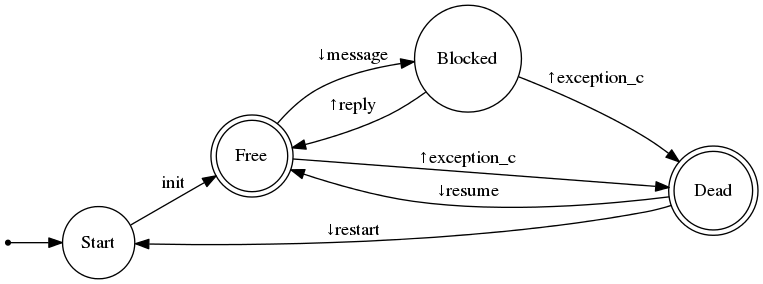
\includegraphics[scale=0.5]{child.png}
%            \caption{A gull}
            \label{fig:1}
        }\\
        \subfigure[Supervisor]{
           \label{fig:2}
           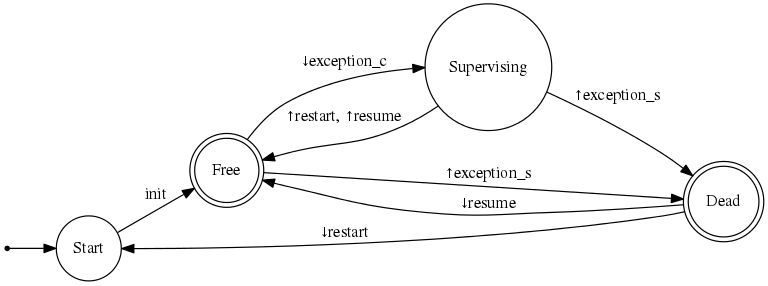
\includegraphics[scale=0.5]{supervisor.png}
        }\\
  \caption{Worker and Supervisor as Deterministic Finite Automata}
  \label{fig:DFA}        
\end{figure}

\subsection{Implementation Considerations}

The two DFAs given in Figure \ref{fig:DFA} are abstracted for theoretical 
study.  In an implementation of the supervision tree model, following issues 
might be considered.

\paragraph{Distributed Deployment}
Supervision Tree represents the logic relationship between nodes.  In 
practice, nodes of a supervision tree may be deployed in distributed machines.  
A child node may be restarted at or shipped to another physical or virtual 
machine but stays in the same place in the logic supervision tree.


\paragraph{Heart-Beat Message}  At run-time, failures may occur at any time for 
different reasons.  In some circumstances, failure messages of a child may not 
be delivered to its supervisor, or even worse, not sent by the failed child at 
all.  To built a system tolerant to the above failures, supervisors need to be 
aware of the liveness of their children.  One approach to achieve this is 
asking the child periodically sending heart-beat message to its supervisor.  
If no heart-beat message is received from a child for some consecutive 
periods, that child is considered dead by the supervisor and an appropriate 
recovery process is activated.  In the model, a 
logical exception is sent from a child to its supervisor when no heart-beat 
message is delivered within a time-out, and a restart or resume message is sent 
to a suitable machine where the node will reside.


\paragraph{Message Queuing}
In the simplified model given in Figure \ref{fig:1}, a worker can processed one 
message a time when it is {\bf Free}.  The model does not exclude the case 
where messages are queuing either in memory or a distributed database.  
Similarly, when a worker is resumed from the failure of processing a message, 
the message it was processing may be retrieved from a cache or be discarded.




\subsection{Unifying Supervisor and Worker}

Notice that the model for supervisor and worker are similar if exceptions from 
the child is viewed as request messages to a supervisor and restart/resume 
is viewed as reply messages to a child.  Can we defined a $combined$ node which 
can be both a worker for a task and a supervisor for some children? Of course 
we can, as what have been implemented in Akka\citep{akka_doc} and inherited by 
TAkka. The rest of this sub-section will compare three strategies of unifying 
supervisor and worker.

\paragraph{Supervisor as a Worker}  In the design of Akka, messages to 
actors are not typed.  An Akka actor therefore can be both a supervisor and a 
worker.  To model an Akka actor, only Figure \ref{fig:1} is required.

\paragraph{Combining Supervisor and Worker}  The TAkka library inherits the 
implementation of Akka, but separates messages for supervision purpose from 
messages for general purposes so that an actor can be parameterized by the 
type of message it expects.  A more precise model for a TAkka actor is given in 
Figure \ref{fig:3}.  Both Akka actor and TAkka actor can only be a supervisor 
or a worker at a time.  As a result, the supervision task may be blocked until 
the end of another computational task.


\paragraph{Supervisor in Parallel with Worker}  One way to get around the 
limitation of Akka and TAkka's design is place the supervision process and the 
worker process in parallel, as shown in Figure \ref{fig:4}.  From the 
perspective of model analysis, the above parallel model is equivalent to the 
one which separates the supervisor process and the worker process into two 
nodes, and treat them as siblings or a supervisor and a child.



\begin{figure}
%  \ContinuedFloat 
  \centering         
        \subfigure[Supervisor AND Worker]{
            \label{fig:3}
            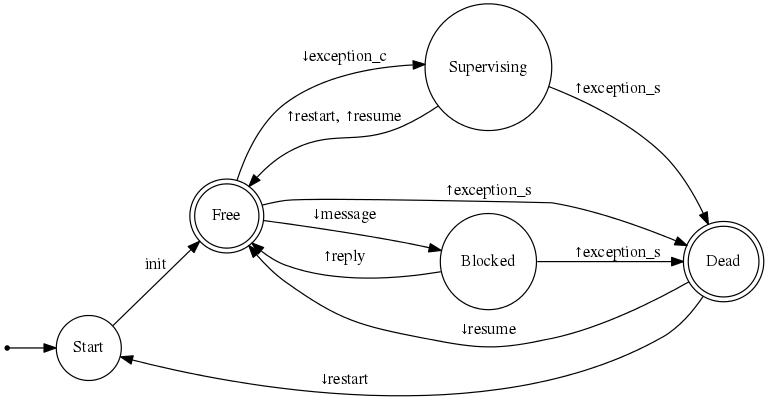
\includegraphics[scale=0.5]{supervisorANDchild.png}
        }\\
        \subfigure[Supervisor PAR Worker]{
            \label{fig:4}
            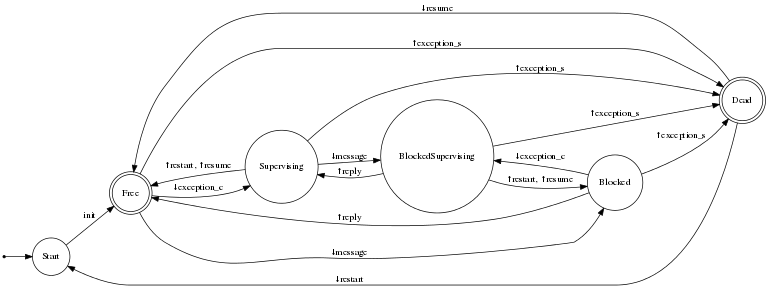
\includegraphics[scale=0.5]{supervisorPARchild.png}
        }\\
    \caption{A Node that Unifies Supervisor and Worker}
   \label{fig:unify}
\end{figure}


To summarize, a node that naively combining the role of supervisor and worker 
(Figure \ref{fig:1} and \ref{fig:3}) has less availability than a node that 
place the supervision process and the worker process in parallel processes 
(Figure \ref{fig:4}).  Interestingly, during the process of designing TAkka, we 
realized that the type of supervision messages should be separated 
from the type of other messages.  However, partly because we would like to 
reuse the Akka implementation and partly because we did not have the above 
model at that time, the process of handling supervision messages is not 
separated from the process of handling other messages.


\subsection{Reliability of a Node}

The reliability of a node, either a worker or a supervisor, is defined as:

The the probability that a node is in the {\bf Free} state.


\subsection{Reliability of a Supervision Tree}

A supervision tree in this proposal consists of workers and supervisors defined 
in Figure \ref{fig:1} and Figure \ref{fig:2} respectively.  A node that 
combines a supervisor and a worker is separated into two nodes, together with a 
constraint that one node will fail when the other fails.

The reliability of a supervision tree may be derived from following factors:

\begin{itemize}
  \item The reliabilities of all workers.  Although testing the reliability of 
a system with low failure rate is difficult or even impractical, the 
reliability of an individual component may be measured within a reasonable 
short time. 
  \item The reliability of a supervisor.  The reliability of a supervisor 
process may be tested as part of the library development process.
  \item The relationship between nodes.  Nodes in a supervision tree may 
collaborate to perform a task or to achieve a higher reliability. The 
reliability of a supervising shall capture complex relationships 
between nodes.
\end{itemize}

The experiment proposed in section \ref{iterative} may to used to measure the 
reliabilities of individual nodes in a supervision tree.  To obtain the 
reliability of a supervision tree, when direct measurement becomes impractical, 
knowledge about constraints between nodes are required.  

I propose to investigate following problems in the next stage:

\begin{itemize}
  \item What are possible constraints between nodes?  For each constraint, what 
is the algebraic relationship between the reliability of a sub-tree and 
reliabilities of individual nodes?
  \item Based on the above result, how to calculate the overall reliabilities 
of a supervision tree?  When is the reliability is improved by using 
supervising tree, and when not?
  \item Given the reliabilities of individual workers and constraints between 
them, is there an algorithm to give a supervision tree that improves the 
reliability?  If not, can we determine if the desired reliability is not 
achievable? 
\end{itemize}


\bibliographystyle{abbrvnat}
\bibliography{reliability}

\end{document}